\documentclass[class=report, crop=false, 12pt,a4paper]{standalone}
\usepackage{enumitem}
\usepackage{tikz}
\usepackage{float}
\usepackage{graphicx}
\usepackage{siunitx}
\begin{document}
A \textbf{control system} is a mechanism which alters the future state of a particular system. \textbf{Control theory} is the method of selecting appropriate inputs. Control theory usually concerns dynamic behaviour of physical systems - the goal is to design a controller which leads to the system exhibiting the desired behaviour. Control systems have a large range of applications throughout engineering such as autopilot systems for ships and aircraft, radar tracking, robotics, machinery plant control and machine tools. 
\subsection*{Methodology}
\begin{itemize}
  \item \textbf{Modelling} - Mathematical model of a system or "transfer function." Comes from detailed analysis of a system and often involves simplifications
  \item \textbf{Prediction} - The model is used to predict the behaviour of the system for a range of parameters and expected excitations
  \item \textbf{Design} - Design a controller which achieves its operating objectives and test it on the model
  \item \textbf{Test} - Here, theory is taken into reality and we compare our model to the physical hardware. Testing of the validity of our assumptions also takes place
  \item \textbf{Iterate} - Improve controller design through updated models
\end{itemize}
\section{Open loop control}
In an \textbf{open loop} control system, the input to the system is not dependant on any previous outputs. The output of the system is not being observed to confirm whether the desired output has been achieved. 
\begin{figure}[H]
  \centering
  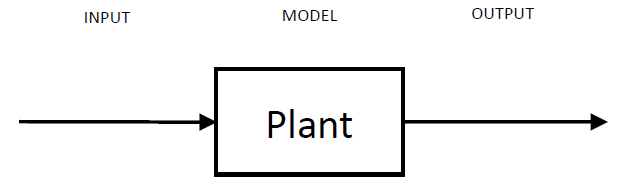
\includegraphics[width = 0.8\textwidth]{../img/openloopcontrol.png}
\end{figure}
These control systems are simple and low cost. They are used in systems where feedback is not important. For example, a washing machine runs for 90 minutes, regardless of whether the clothes are dry after 60 minutes. 
\subsection*{3D Printer example}
Consider the stepper motors used to move the print head in x and y with belt and pulley system. Here, open loop control is used because the stepper motors are simple to control and have a relationship between input and output. For example, consider a stepper motor which moves 0.2\si{\milli\m} each step (S) for an integer number of steps. 
\begin{figure}[H]
  \centering
  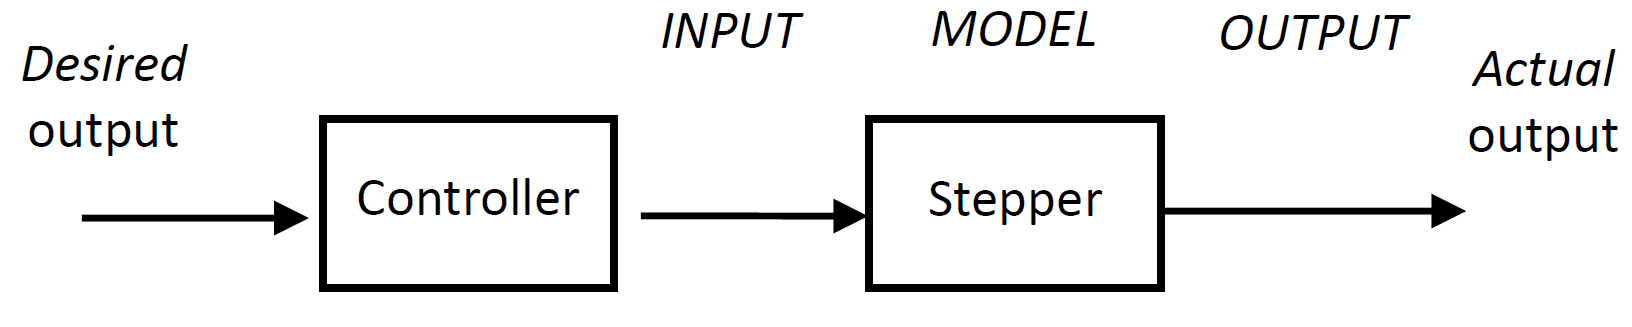
\includegraphics[width = 0.8\textwidth]{../img/controlstrat3dprinter.png}
\end{figure}
Implementing such a controller could be done with the following pseudocode:
\begin{verbatim}
  Function MovePrintHeadX(Input_mm)
  //convert to number of steps needed
  Steps_S = Input_mm / 0.2
  //send step command to motor
  Stepper.step(Steps_S)
\end{verbatim}
However, the assumption used to model our system is only valid if the stepper motors is within its specification i.e. friction, load, temperature, power are all nominal. As stated before, the system does not observe if the steps were successful or not. 
\section{Closed loop control}
By observing the output and comparing it against your desired output, it is possible to update the input to the system. The observed output is called the \textbf{feedback signal}.
\begin{figure}[H]
  \centering
  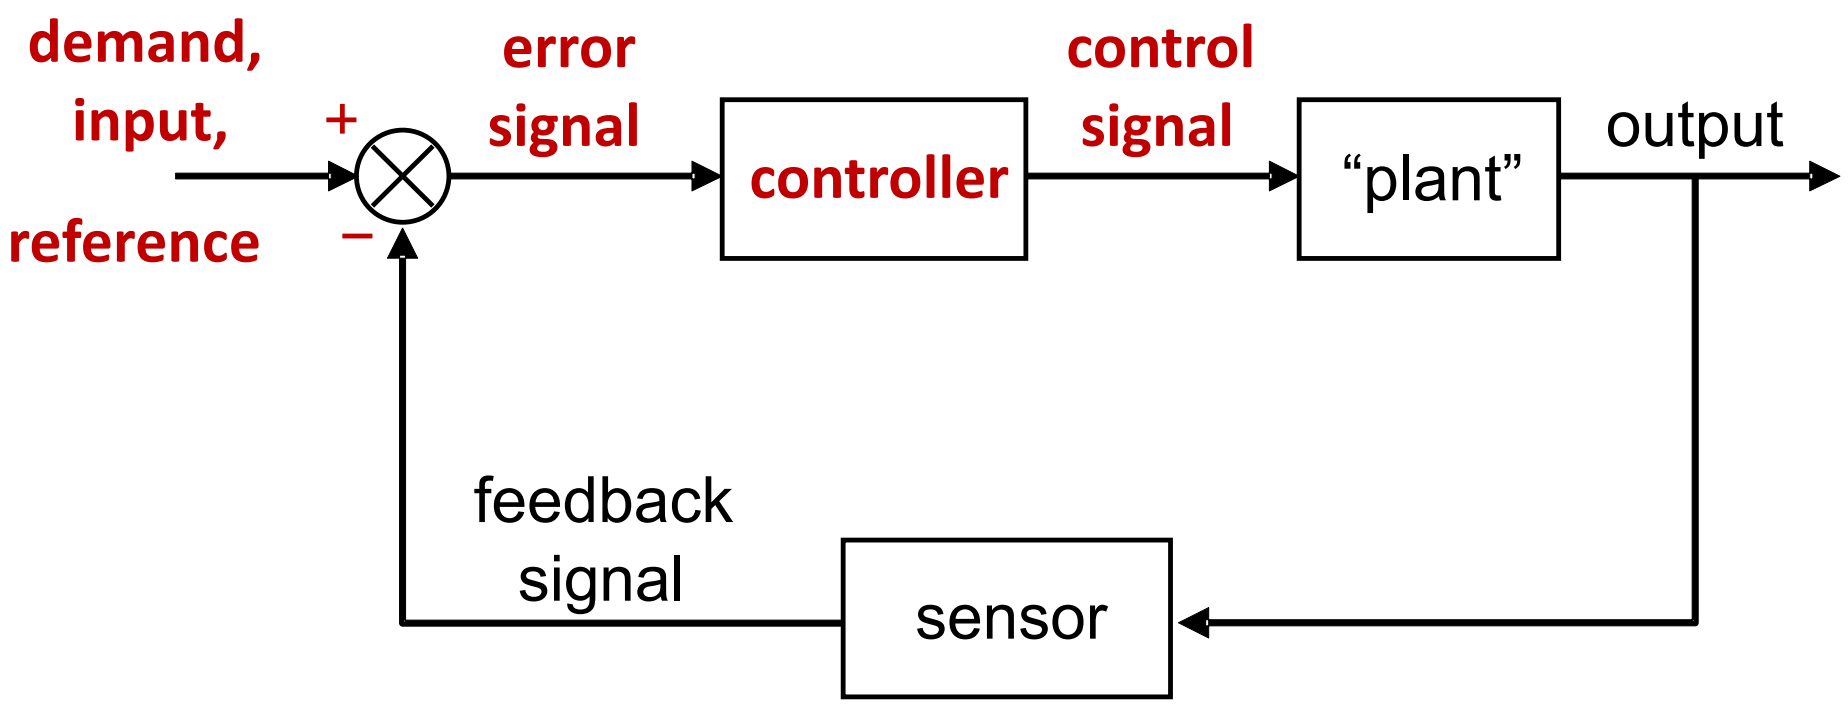
\includegraphics[width = 0.8\textwidth]{../img/closedloopcontrol.png}
\end{figure}
The difference between the desired output and the feedback signal is known as the \textbf{error signal}. This is the signal that the controller uses. Feedback signals allow powerful controllers to be designed.

Taking our 3D printer for example, we can add a position sensor on the x-axis.
\begin{figure}[H]
  \centering
  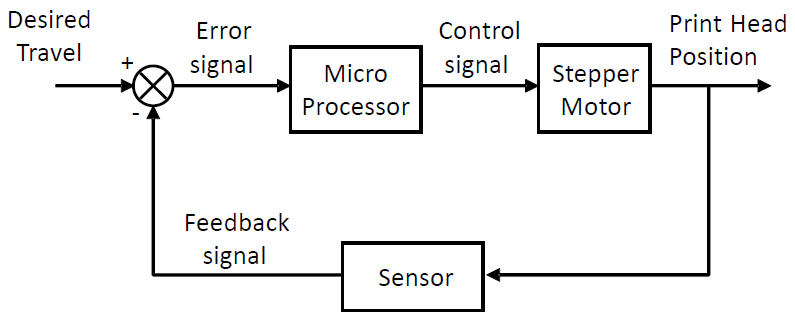
\includegraphics[width = 0.8\textwidth]{../img/controlstrat3dprinterclosed.png}
\end{figure}
The pseudocode for this system could look like this
\begin{verbatim}
  while
    // get measurement of position
    measured_value_mm = Sensor.getValue
    // calc error signal
    error_mm = setpoint_mm - measure_value_mm
    // convert to steps
    Steps_S - error_mm / 0.2
    // send step command to motor
    Stepper.Step(Steps_S)
  end
\end{verbatim}
We must consider whether this extra complexity is required or necessary in our system. Closed loop systems are not a magic bullet; they require careful modelling to predict system behaviour and a considered choice of parameters to prevent the system becoming unstable. 
\section{Block diagram representation of control loops}
\begin{figure}[H]
  \centering
  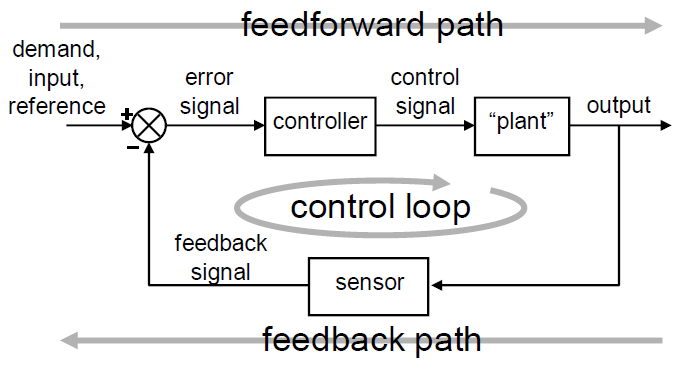
\includegraphics[width = 0.8\textwidth]{../img/blockdiagram1.png}
\end{figure}
Control systems are often represented by block diagrams which show the information flow.
\begin{figure}[H]
  \centering
  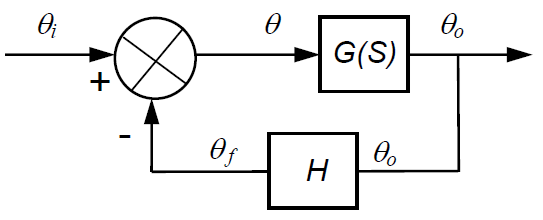
\includegraphics[width = 0.8\textwidth]{../img/blockdiagram2.png}
\end{figure}
\textbf{Flow path} indicates the direction of data flow (from left to right). Values are maintained at a branch.
\begin{figure}[H]
  \centering
  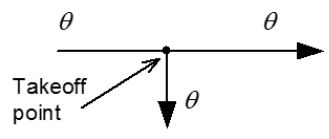
\includegraphics[width = 0.5\textwidth]{../img/flowpath.png}
  \caption{Flow path}
\end{figure}
\textbf{Function block}. The functions acts on the input to to produce the output. $x_{out} = f(x_{in})$
\begin{figure}[H]
  \centering
  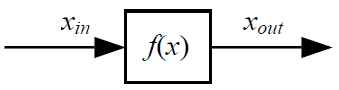
\includegraphics[width = 0.5\textwidth]{../img/functionblock.png}
  \caption{Function block}
\end{figure}
\textbf{Comparator}. The signals $\theta_1$ and $\theta_2$ are compared according to the signs (+ or -) and the result is $\theta_3$. They \textbf{must} have the same units. In this case $+\theta_1 - \theta_2 = \theta_3$.
\begin{figure}[H]
  \centering
  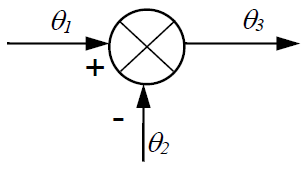
\includegraphics[width = 0.5\textwidth]{../img/comparator.png}
  \caption{Comparator}
\end{figure}
\begin{figure}[H]
  \centering
  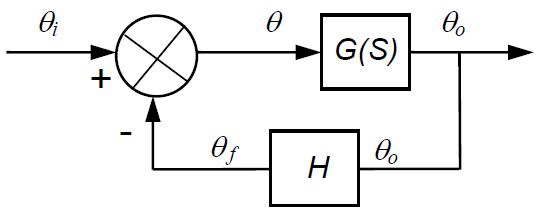
\includegraphics[width = 0.8\textwidth]{../img/blockdiagram3.png}
\end{figure}
\section{Basic definitions/concepts}
The following definitions are based on the standards of the IEEE (Institute of Electrical and Electronics Engineers)
\begin{itemize}
  \item A \textbf{system} is an arrangement, set or collection of components connected or related in such a manner as to form an entirety or whole.
  \item A \textbf{control system} is an arrangement of physical components connected or related in such a manner as to command, direct or regulate itself or another system. The components act together to perform a function not possible with any of the individual parts. 
  \item The \textbf{input} is the stimulus or excitation applied to a system usually in order to produce a specified response.
  \item The \textbf{output} is the actual response obtained.
  \item An \textbf{open loop control system} is one in which the input is independent of the output.
  \item A \textbf{closed loop control system} is one in which the input is somehow dependent on the output.
  \item \textbf{Error signal} (or \textbf{actuating signal}) is the difference between the reference input and the feedback, in closed loop control systems it is this signal which is sent to the plant not the reference signal.
\end{itemize}
\section{Notation}
Large complex systems can be broken down into interconnected smaller ones and reduced further into a number of blocks. 
\begin{figure}[H]
  \centering
  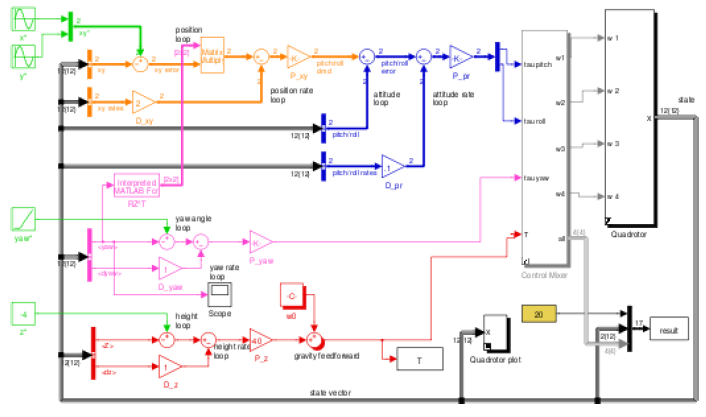
\includegraphics[width = 0.8\textwidth]{../img/quadcopterexampleblock.png}
  \caption{A quadcopter with lots of PID controllers running in parallel. Each colour represents a control loop for position, altitude, yaw etc.}
\end{figure}
Complex systems can be abstracted to a signal block if the behaviour can be adequately modelled. Consider modelling the stepper motor from the 3D printer, in reality a complex device, as a single block. This is analogous to representing a complex op-amp circuit as a single unit.
\begin{figure}[H]
  \centering
  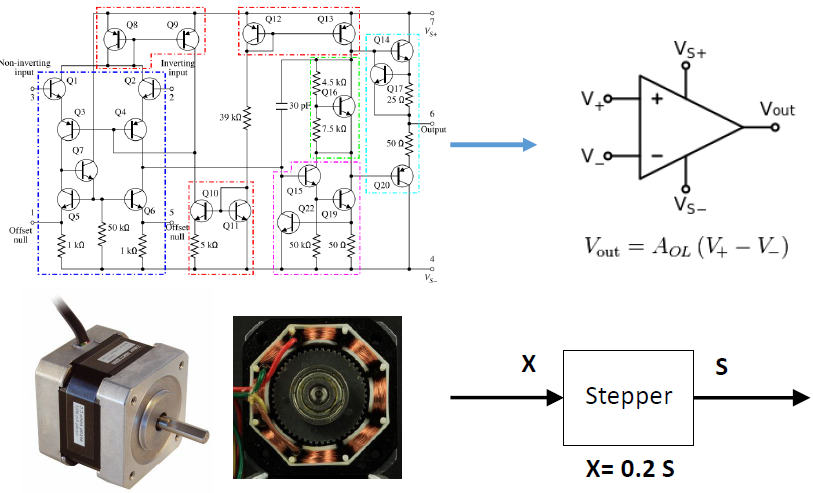
\includegraphics[width = 0.8\textwidth]{../img/blockdiagram4.png}
\end{figure}
\section{Summary}
\begin{itemize}
  \item Control systems are interconnected components which are configured to provide a desired response.
  \item Two broad categories of control systems: open loop (no feedback of output) and closed loop (feedback signal).
  \item Successful design of the controller requires consideration of the design goals, definition of the specifications, system definition, modelling and subsequent analysis. Controller design is an iterative process.
\end{itemize}
\end{document}